\section{Auswertung}
\label{sec:Auswertung}

\subsection{Einzelspalt}
Die zu Beginn bestimmten Werte für die Spaltbreite sowie die angegebenen Werte des Herstellers sind in \ref{tab:b} angegeben.

\begin{table}
  \caption{Werte für die mit dem Mikroskop gemessene Spaltbreite der drei Einzelspalte und die Angaben des Herstellers.}
  \centering
  \label{tab:b}
  \begin{tabular}{c c c c}
    \toprule
   - & $b_1/\si{\milli\meter}$ & $b_2/\si{\milli\meter}$ & $b_3/\si{\milli\meter}$ \\
   \midrule
   Hersteller & 0.075 & 0.15 & 0.4 \\
   Mikroskop & 0.1 & 0.156 &  0.385\\
   \bottomrule
   \end{tabular}
\end{table}

Eine weitere Möglichkeit die Spaltbreite zu ermitteln, besteht darin, den Winkel $\phi$ gegen die Stromstärke $I$ aufzutragen. Von den Stromstärken in Tabelle \ref{tab:messwerte} wird jeweils der zu Anfang gemessene Dunkelstrom $I_\mathrm{D}=0.55\si{\nano\ampere}$ abgezogen. Um aus $d$ in Tabelle \ref{tab:messwerte} den Winkel $\phi$ zu berechnen, wird folgende Formel verwendet:
\begin{equation}
  \label{eqn:winkel}
  \phi \approx \frac{d-d_0}{L}.
\end{equation}
Dabei ist $d_0=25 \si{\milli\meter}$ die Stelle der Mitte des Hauptmaximums und $L$ der Abstand zwischen Spalt und Detektor.
Mit Hilfe einer Ausgleichsrechnung wird der Parameter $b$ für die Spaltbreite bestimmt.

\begin{table}
  \caption{Messwerte für die Stromstärke $I$ in Abhängigkeit von der Verschiebung $d$ für die drei Einzelspalte.}
  \centering
  \label{tab:messwerte}
  \footnotesize
  \begin{tabular}{c c c c}
    \toprule
   $d/\si{\milli\meter}$ & $I_3$/$\mu$\si{\ampere} & $I_2/\si{\nano\ampere}$ & $I_1/\si{\nano\ampere}$ \\
   \midrule
25.0 & 15.5 & 2050 &250 \\
24.5 & 11.0 & 2000 & 250 \\
24.0 & 5.5  & 1880 & 245 \\
23.5 & 1.3  & 1650 & 237 \\
23.0 & 0.36 & 1400 & 230 \\
22.5 & 0.65 & 1100 & 220 \\
22.0 & 0.58 & 820 & 210 \\
21.5 & 0.245 & 560 & 200 \\
21.0 & 0.16 & 330 & 185 \\
20.5 & 0.295 & 180 & 170 \\
20.0 & 0.290 & 79 & 155 \\
19.5 & 0.150 & 26.5 & 140 \\
19.0 & 0.086 & 13.0 & 125 \\
18.5 & 0.115 & 25.5 & 110 \\
18.0 & 0.105 & 50 & 96 \\
17.5 & 0.064 & 72 & 82 \\
17.0 & 0.068 & 88 & 69 \\
16.5 & 0.094 & 91 & 58 \\
16.0 & 0.080 & 81 & 48 \\
15.5 & 0.046 & 65 & 38 \\
15.0 & 0.044 & 45 & 30 \\
14.5 & 0.061 & 27.0 & 23 \\
14.0 & 0.054 & 13.5 & 17 \\
13.5 & 0.035 & 7.6 & 12.5 \\
13.0 & 0.035 & 8.4 & 9.1 \\
12.5 & 0.042 & 14  & 6.6 \\
25.5 & 15.0 & 2075 & 255 \\
26.0 & 9.8  & 1950 & 250 \\
26.5 & 4.1  & 1750 & 245 \\
27.0 & 0.88 & 1475 & 236 \\
27.5 & 0.40 & 1200 & 230 \\
28.0 & 0.64 & 880 & 217 \\
28.5 & 0.46 & 630 & 205 \\
29.0 & 0.150 & 400 & 195 \\
29.5 & 0.135 & 230 & 180 \\
30.0 & 0.240 & 110 & 165 \\
30.5 & 0.203 & 43 & 150 \\
31.0 & 0.103 & 15 & 135 \\
31.5 & 0.094 & 16.5 & 120 \\
32.0 & 0.120 & 50 & 105 \\
32.5 & 0.086 & 64 & 90 \\
33.0 & 0.042 & 70 & 76 \\
33.5 & 0.051 & 56 & 64 \\
34.0 & 0.072 & 41 & 52 \\
34.5 & 0.060 & 26.5 & 42 \\
35.0 & 0.046 & 15.0 & 34 \\
35.5 & 0.058 & 6.0 & 27 \\
36.0 & 0.065 & 6.0  & 20.5 \\
36.5 & 0.046 & 7.7  & 15.5 \\
37.0 & 0.027 & 11.5 & 11.0 \\
37.5 & 0.032 & 15.5 & 8.3 \\
\bottomrule
\end{tabular}
\end{table}

\begin{figure}
  \centering
  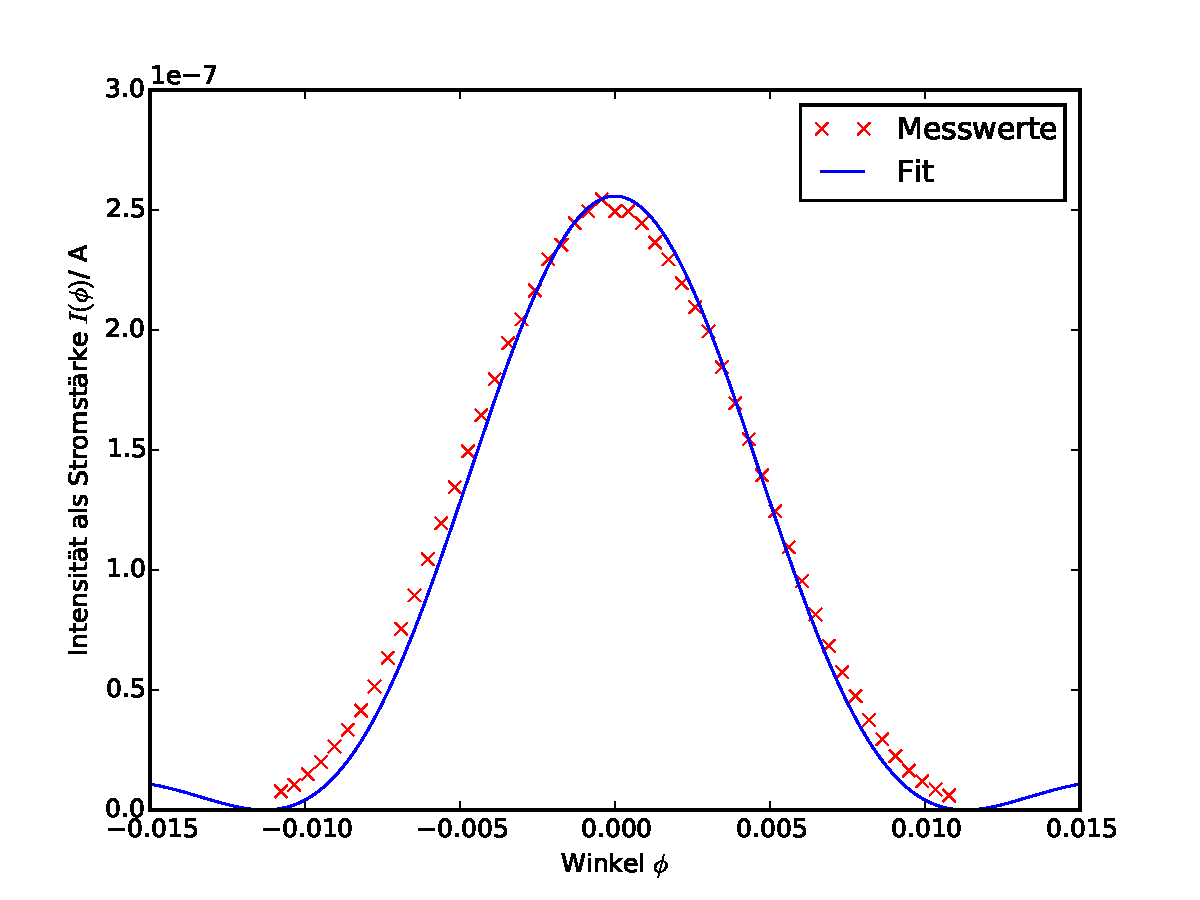
\includegraphics[scale=0.6]{build/einzel1.pdf}
  \caption{Intensität als Stromstärke $I$ in Abhängigkeit vom Winkel $\phi$ für den kleinsten Spalt.}
  \label{fig:einzel1}
\end{figure}

\begin{figure}
  \centering
  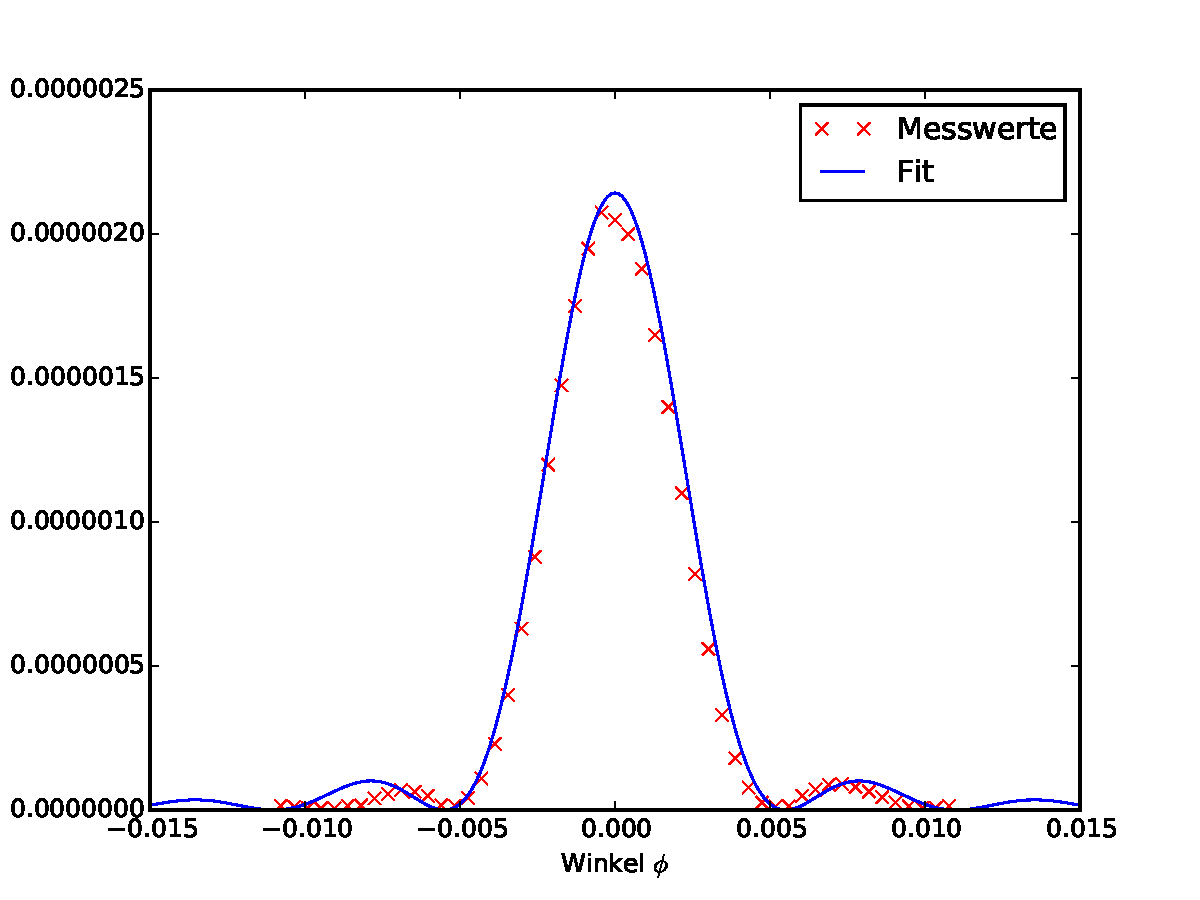
\includegraphics[scale=0.6]{build/einzel2.pdf}
  \caption{Intensität als Stromstärke $I$ in Abhängigkeit vom Winkel $\phi$ für den zweitgrößten Spalt.}
  \label{fig:einzel2}
\end{figure}

\begin{figure}
  \centering
  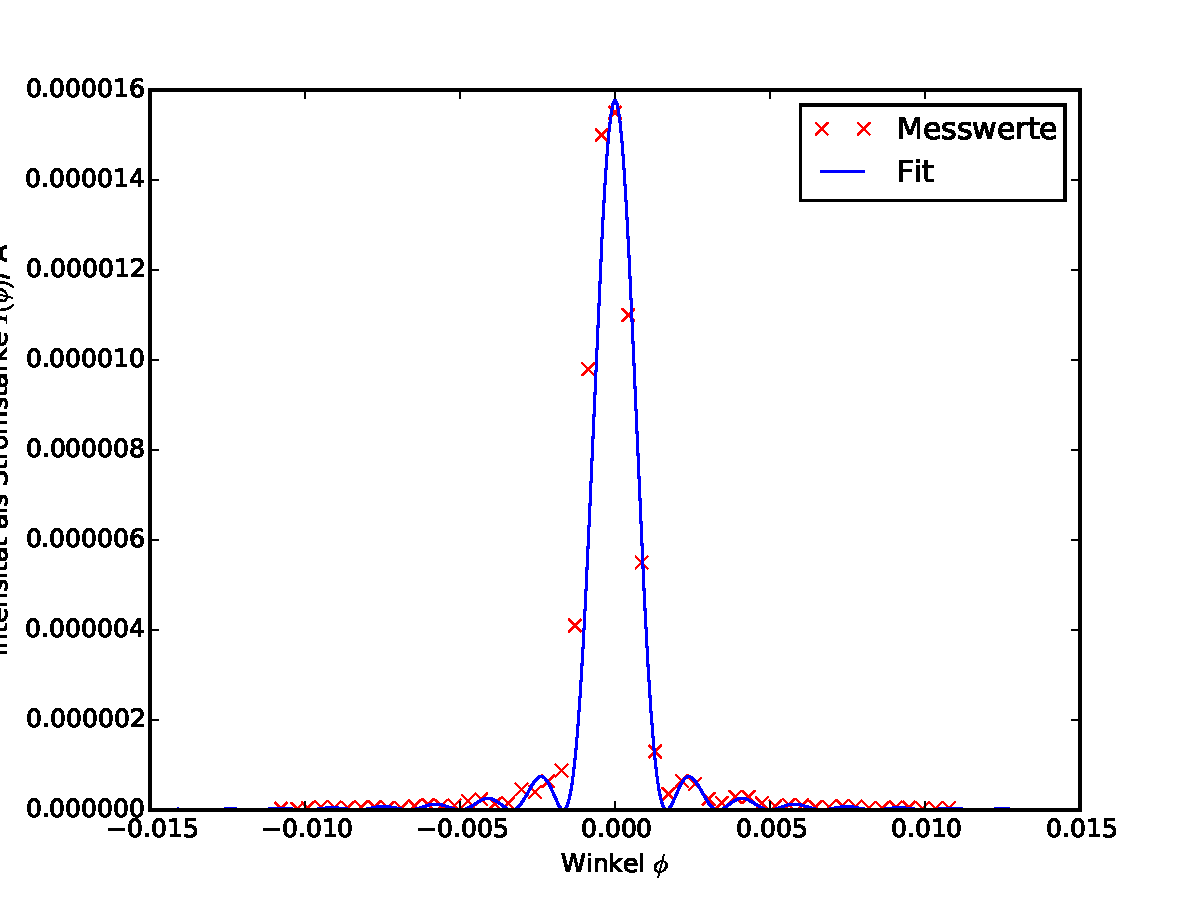
\includegraphics[scale=0.6]{build/einzel3.pdf}
  \caption{Intensität als Stromstärke $I$ in Abhängigkeit vom Winkel $\phi$ für den größten Spalt.}
  \label{fig:einzel3}
\end{figure}

Für die Einzelspalte wird jeweils Gleichnung \ref{eqn:einzel} als Fitfunktion verwendet. In Abbildung \ref{fig:einzel1} bis \ref{fig:einzel3} sind Intesitätsverteilungen der Einzelspalte grapisch dargestellt.
Für die Spaltbreiten $b$ und $A$ ergibt sich mit Hilfe der Ausgleichsrechnung:
\begin{align}
  b_1 &= 0.056 \si{\milli\meter} \\
  A_1 &= 5.1 \\
  b_2 &= 0.115 \si{\milli\meter}\\
  A_2 &= 3.5 \\
  b_3 &= 0.38 \si{\milli\meter} \\
  A_3 &= 27.5 \\
\end{align}

Um beurteilen zu können, welche der Methoden zur Bestimmung der Spaltbreite genauer ist, werden die ermittelten Werte miteinander verglichen. Dazu werden die prozentualen Abweichungen von den Herstellerangaben berechnet, welche in Tabelle \ref{tab:abweichungen} zu finden sind.

\begin{table}
  \caption{Prozentuale Abweichungen der ermittelten Spaltbreiten.}
  \centering
  \label{tab:abweichungen}
  \begin{tabular}{c c c c c c c}
    \toprule
   - & $b_1/\si{\milli\meter}$ & Abweichung /\% & $b_2/\si{\milli\meter}$ & Abweichung /\% & $b_3/\si{\milli\meter}$ & Abweichung /\%\\
   \midrule
Hersteller & 0.075 & - & 0.15 & - & 0.4 & -  \\
Mikroskop & 0.1 & 33.3 & 0.156 & 4.0 & 0.385 & 3.9\\
Beugung & 0.056 & 33.92 & 0.115 & 30.43 &  0.38 & 5.26 \\
  \bottomrule
  \end{tabular}
  \end{table}

  \subsection{Doppelspalt}
  Für Spaltbreite $b$ und den Abstand der Spalte $s$ bei der Messung mit dem Mikroskop ergeben sich die Werte in Tabelle \ref{tab:s}.

\begin{figure}
  \centering
  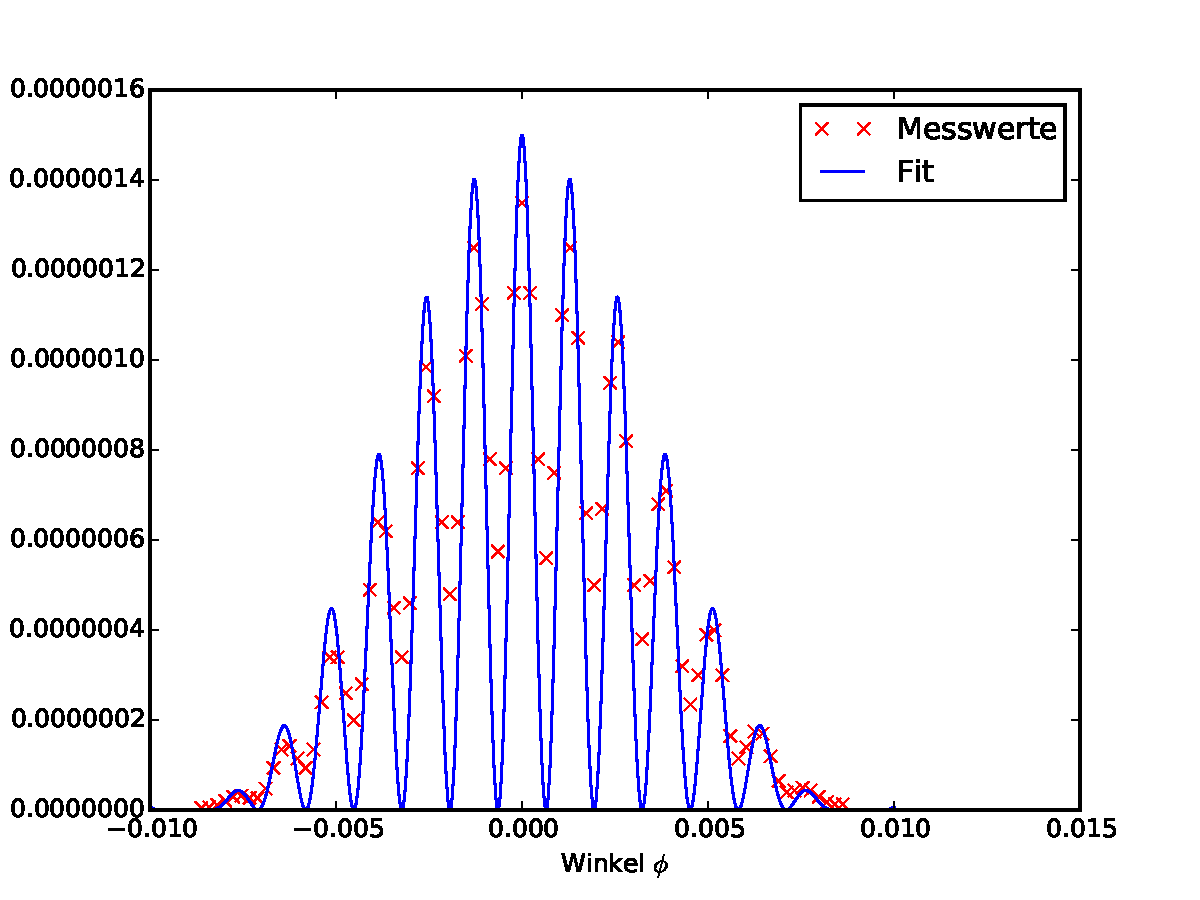
\includegraphics[scale=0.6]{build/doppel.pdf}
  \caption{Intensität als Stromstärke $I$ in Abhängigkeit vom Winkel $\phi$ für den Doppelspalt.}
  \label{fig:doppel}
\end{figure}

  \begin{table}
    \caption{Werte für die mit dem Mikroskop gemessene Spaltbreite $b$ und die Abstände der Spalte $s$ und Herstellerangaben.}
    \centering
    \label{tab:s}
    \begin{tabular}{c c c}
      \toprule
     - & $b/\si{\milli\meter}$ & $s/\si{\milli\meter}$\\
     \midrule
     Hersteller & 0.1 & 0.4 \\
     Mikroskop & 0.125 & 0.455 \\
     \bottomrule
     \end{tabular}
  \end{table}

  Die Messwerte zur Intensität in Abhängigkeit der Verschiebung $d$ für den Doppelspalt befinden sich in Tabelle \ref{tab:messwerte2}.

  \begin{table}
    \caption{Messwerte zur Intensität in Abhängigkeit von der Verschiebung beim Doppelspalt.}
    \centering
    \label{tab:messwerte2}
    \begin{tabular}{c c | c c}
      \toprule
$d$ / \si{\milli\meter} & $I$ /\si{\nano\ampere} & $d$ / \si{\milli\meter} & $I$ /\si{\nano\ampere}\\
     \midrule
25.00 & 1350	& 25.25 & 1150 \\
24.75 & 1150	& 25.50 & 760 \\
24.50 & 780	& 25.75 & 575 \\
24.25 & 560	& 26.00 & 780 \\
24.00 & 750	& 26.25 & 1125 \\
23.75 & 1100	& 26.50 & 1250 \\
23.50 & 1250	& 26.75 & 1010 \\
23.25 & 1050 &	27.00 & 640 \\
23.00 & 660	& 27.25 & 480 \\
22.75 & 500	& 27.50 & 640 \\
22.50 & 670	& 27.75 & 920 \\
22.25 & 950	& 28.00 & 985 \\
22.00 & 1040	& 28.25 & 760 \\
21.75 & 820	& 28.50 & 460 \\
21.50 & 500	& 28.75 & 340 \\
21.25 & 380	& 29.00 & 450 \\
21.00 & 510	& 29.25 & 620 \\
20.75 & 680	& 29.50 & 640 \\
20.50 & 710	& 29.75 & 490 \\
20.25 & 540	& 30.00 & 280 \\
20.00 & 320	& 30.25 & 200 \\
19.75 & 235	& 30.50 & 260 \\
19.50 & 300	& 30.75 & 340 \\
19.25 & 390	& 31.00 & 340 \\
19.00 & 400	& 31.25 & 240 \\
18.75 & 300	& 31.50 & 135 \\
18.50 & 165	& 31.75 & 94 \\
18.25 & 115	& 32.00 & 115 \\
18.00 & 140	& 32.25 & 143 \\
17.75 & 175	& 32.50 & 135 \\
17.50 & 170	& 32.75 & 94 \\
17.25 & 120	& 33.00 & 48 \\
17.00 & 65 & 	33.25 & 27 \\
16.75 & 40 &	33.50 & 27.5 \\
16.50 & 44 &	33.75 & 32 \\
16.25 & 50 &	34.00 & 30 \\
16.00 & 44 &	34.25 & 20.5 \\
15.75 & 30 &	34.50 & 11.5 \\
15.50 & 18	& 34.75 & 6.4 \\
15.25 & 13.5	& 35.00 & 5.0 \\
15.00 & 13.0	\\
\bottomrule
\end{tabular}
\end{table}

Auch hier muss von der gemessenen Stromstärke aus Tabelle \ref{tab:messwerte} der Dunkelstrom $I_\mathrm{D}$ subtrahiert werden. Die Winkel lassen sich analog zum Einzelspalt nach Gleichung \ref{eqn:winkel} berechnen. Auch hier wird die Stromstärke $I$ gegen den Winkel $\phi$ aufgetragen (siehe Abbildung \ref{fig:doppel}). Mittels einer Ausgleichsrechnung werden die Spaltbreite $b$ sowie der Abstand der Spalte $s$ bestimmt. Als Fitfunktion wird Gleichung \ref{eqn:doppel} verwendet.
Für die Parameter $A$, $b$ und $s$ folgt:
\begin{align}
  A&=1.5 \cdot 10^{-6} \\
  b&=0.07 \si{\milli\meter} \\
  s&=0.49 \si{\milli\meter} \\
\end{align}

Zum Vergleich wird erneut die prozentuale Abweichung berechnet, welche in Tabelle \ref{tab:abweichung2} dargestellt ist.

\begin{table}
  \caption{Abweichungen der ermittelten Spaltbreite $b$ und dem Abstand $s$ mittels Mikroskop und Beugung von den Herstellerangaben.}
  \centering
  \label{tab:abweichung2}
  \begin{tabular}{c c c c c}
    \toprule
   - & $b/\si{\milli\meter}$ & Abweichung/\% & $s/\si{\milli\meter}$ & Abweichung/\%\\
   \midrule
   Hersteller & 0.1 & - & 0.4 & -\\
   Mikroskop & 0.125 & 25.00 & 0.455 & 13.75 \\
   Beugung & 0.07 & 42.86 & 0.49 & 22.50 \\
   \bottomrule
   \end{tabular}
\end{table}
